\documentclass[USenglish]{scrartcl}

\usepackage{a4wide}
\usepackage[T1]{fontenc}
\usepackage[latin1]{inputenc}
\usepackage{epsfig}
\usepackage[pagewise]{lineno}
\usepackage{ae}
\usepackage{listings}
\usepackage{url}
\usepackage{hyperref}
\usepackage{setspace}   % to adjust line spacing


\lstset{% set listing parameters
	language=sh,		% code in shell
	breaklines=true,	%
	linewidth=\textwidth,	% base line width for listings
	showstringspaces=false,	% do not show spaces in strings
	showspaces=false,	% do not show spaces in the code
	basicstyle=\scriptsize\ttfamily,
	commentstyle=\textit,
	framextopmargin=10pt,	% top margin frame
	framexbottommargin=10pt,% bottom margin frame
	frame=tb}		% frame at top and bottom of the code


% \IfFileExists{url.sty}{\usepackage{url}}
%                        {\newcommand{\url}{\texttt}}

% \makeatletter

%%%%%%%%%%%%%%%%%%%%%%%%%%%%%% LyX specific LaTeX commands.
\newcommand{\noun}[1]{\textsc{#1}}

\usepackage{babel}
% \makeatother
\begin{document}

\title{A Tiny Queuing System for \noun{Blast} Servers}


\author{\noun{Colas Schretter}\footnote{cschrett@ulb.ac.be} and \noun{Laurent Gatto}\footnote{lgatto@ulb.ac.be}}

\maketitle

%%%%%%%%%%%%%%%%%%%%%%%%%%%%%%%%%%%%%%%%%%%%%%%%%%%%%%%%%%%%%%%%%%%%%%%%%%%%%%%%%%%%%%%%%%%%%%%%%%%%%
%%%%%%%%%%%%%%%%%%%%%%%%%%%%%%%%%%%%%%%%%%%%%%%%%%%%%%%%%%%%%%%%%%%%%%%%%%%%%%%%%%%%%%%%%%%%%%%%%%%%%

% \linenumbers
\doublespacing

\section*{Introduction}

When multiple \noun{Blast} \cite{blast} similarity searches are run simultaneously against large databases and no parallel computing facility is at hand, the IO-bound process requires to limit the number of concurrent runs. Therefore we setup a queuing system to ensure that, at any time, the executed jobs do not require more than the available IO resources.

Existing queuing systems like OpenPBS \cite{opbs}, Maui \cite{maui} or Sun Grid Engine \cite{sge} could be installed to solve these requirements. However, we developed a set of shell scripts that work together to add lightweight queuing abilities to any \noun{UNIX}-like systems. The features of our solution are:

\begin{itemize}
	\item it only relies on shell scripts and the crontab service
	\item it is easy to install, use and extend
	\item it provides e-mail notifications
\end{itemize}

The set of scripts of a real-case application are given and commented. The example presented has been limited (\textit{i.e.} in the number of \noun{Blast} parameters) for didactical purposes. This document should help anyone to adapt those scripts and extend the system for further requirements.

%%%%%%%%%%%%%%%%%%%%%%%%%%%%%%%%%%%%%%%%%%%%%%%%%%%%%%%%%%%%%%%%%%%%%%%%%%%%%%%%%%%%%%%%%%%%%%%%%%%%%
%%%%%%%%%%%%%%%%%%%%%%%%%%%%%%%%%%%%%%%%%%%%%%%%%%%%%%%%%%%%%%%%%%%%%%%%%%%%%%%%%%%%%%%%%%%%%%%%%%%%%

\section*{Framework}

In the following sections, we describe each functionality by providing the scripts and their dependencies. First, we describe how users submit jobs to the system. Then, we explain how we implemented the queuing mechanism. 

We setup an active system loop that watches for the presence of new job requests and a locking mechanism to limit resources usages. A general deployment diagram describing the queuing system is given in figure \ref{fig}. The requirements for the queuing system are a \noun{UNIX}-like operating system, a running webserver and the necessary \noun{Blast} programs and databases.



\begin{figure}[h]
\begin{center}
	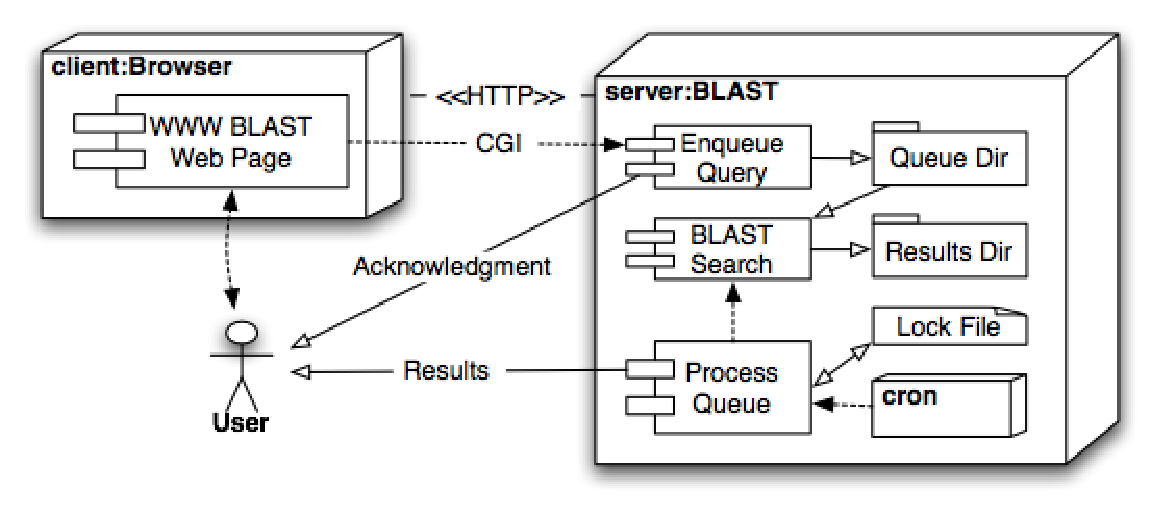
\includegraphics[width=12cm]{tiny_queuing_system_deployment0.eps}
	\caption{Deployment diagram of the queuing system for \noun{Blast} searches.}
	\label{fig}
\end{center}
\end{figure}

\subsection*{Job Submission}

The queueing system manages two sets of files: 
\begin{enumerate}
	\item \noun{Blast} searches ready to be run as soon as resources are freed
	\item result files of recently finished searches
\end{enumerate}
The search results are saved in a web accessible directory (\textit{i.e.} \texttt{/var/www/localhost/htdocs/}). Each file is uniquely identified by its exact generation time and can be consulted by the user. The \textit{ready-to-be-run} searches (consisting of a \texttt{blastall} command and the input queries) are stored in the queue directory. The queuing blast file are identified by their exact generation time and the users contact email adress. Note that the \texttt{blast/queue} and \texttt{blast/results} directories have to be respectively  writable and readable by the apache user.


We use a modified \noun{WWWBlast} web page as entry to the queuing system. The only modification consists in the addition of an HTML text field for the users email adress. When posted, the form invokes a shell cgi script \texttt{queue\_blast\_jobs.sh} located in a directory containing server scripts, typically \texttt{/var/www/localhost/cgi-bin/}. This script will parse the user's blast parameters and add the appropriate file to the blast jobs queue. To avoid a possible delay if resources are free, the \texttt{process\_blast\_jobs.sh} script (see below) is immediately launched (independently of cron). 

\lstinputlisting[caption=queue\_blast\_jobs.sh]{./scripts/queue_blast_jobs.sh}
\bigskip


%%%%%%%%%%%%%%%%%%%%%%%%%%%%%%%%%%%%%%%%%%%%%%%%%%%%%%%%%%%%%%%%%%%%%%%%%%%%%%%%%%%%%%%%%%%%%%%%%%%%%

\subsection*{Job Watcher and Launcher}

A crontab daemon periodically runs the \texttt{process\_blast\_jobs.sh} script that checks if files are stored in the queue directory and eventually runs the \noun{Blast} searches. 
\begin{verbatim}
MAILTO=""
* * * * * /var/www/localhost/htdocs/blast/process_blast_jobs.sh 
\end{verbatim}

In this example, \noun{Blast} queries will be detected in less than a minute. The script first checks if the necessary ressources are available. When an application is running behind the queuing system, a lock file is created as a flag and the script exits. If no lock file is present, \texttt{process\_blast\_jobs.sh} first locks the system. For all the jobs in the queues, it then chooses the oldest job file, recovers the users email adress and the future result file url and launches the similarity search. When a \noun{Blast} search finishes, the script mails the user the result url. When all the jobs in the queue are done, the system is unlocked to allow the next searches to be performed.


\lstinputlisting[caption=process\_blast\_jobs.sh]{./scripts/process_blast_jobs.sh}
\bigskip




\section*{Possible extensions}

It is further possible to distribute the computation charge among several independent and dedicated servers. A possibility would be to have a web server as  the entry-point for job submissions, that manages the queue and result directories. In order to ensures interactive performances to any visitor, the resources of this server are exclusively reserved for dynamic web page generation and mailing capabilities. Resource-consuming tasks are not allowed to run on the web server. Therefore, executables are launched on a third party application server. The shell cgi scripts \texttt{queue\_blast\_jobs.sh} and \texttt{process\_blast\_jobs.sh} would, in such case, still be located on the webserver, but the \noun{Blast} search would be run over \texttt{ssh} on the application server and the results would be copied back to the webserver\footnote{ssh and scp need to be automated with ssh keys to avoid password requests}:

\begin{verbatim}
ssh wwwrun@application_server "$JOB"
scp -q wwwrun@application_server:~/results/$OUTPUT  $QUEUEDIRS/results/.
\end{verbatim}

It is further possible to define two or more simultaneous jobs by allowing two or more \texttt{locked} files to be created. Different \texttt{locked} files may be associated with different application hosts. \texttt{process\_blast\_jobs.sh} would check for the existence of \texttt{locked\_1} to \texttt{locked\_n} before starting a new search.


\bibliographystyle{plain} 
\bibliography{queuerefs}


\end{document}



